%!TEX root = ../report.tex

\chapter{Introduction}
\label{chap:intro}
\newcommand{\chapquote}[3]{\begin{quotation} \textit{#1} \end{quotation} \begin{flushright} - #2\end{flushright} }

\chapquote{``You can't cross the sea merely by standing and staring at the water.''}{Rabindranath Tagore}



More than two-thirds of the earth surface is covered by ocean and other water bodies. For a human, it is often impossible to be able to explore it extensively. 
For finding a new source of energy, monitoring tsunami, global warming or maybe just to learn about deep-sea eco-system or may be to look for a lost ship or an airplane, the need for venturing into potentially dangerous underwater scenarios appear regularly, in fact getting more frequent. That's why more and more robots are being deployed in underwater scenarios and a lot of research is going in this direction.
Some of the exploration or monitoring tasks require the robot to see underwater, to make intelligent decisions.
But the underwater environment is very difficult for optical cameras, as light is attenuated and absorbed by the particles in the water. And a lot of real-life monitoring and mapping tasks take place in a cluttered and turbid underwater scenario. The limited visibility range (underwater) of an optical sensor is a big challenge. Hence sonar is a more practical choice for underwater sensing as the sound can travel 
long distances with comparatively little attenuation.

An underwater robot, equipped with sonar image sensors, regularly needs to perform basic tasks such as object detection and recognition, navigation, manipulation etc. For most of it, effective acoustic vision is fundamental. 
In underwater scenarios, sonar patch matching functionality is very useful in various applications such as data association in simultaneous localization and mapping (SLAM), object tracking, sonar image mosaicing \cite{hurtos2012fourier}
etc. Patch matching, in general, is heavily used in computer vision and image processing applications for low-level tasks like image stitching \cite{brown2007automatic}, 
deriving structure from motion \cite{molton2004locally}, also in high-level tasks such as object instance recognition \cite{lowe1999object}, object classification \cite{yao2012codebook}, multi-view reconstruction \cite{seitz2006comparison}, 
image-retrieval etc. 
Typical challenges in patch matching tasks are different viewing points, variations in illumination of the scene, occlusion, and different sensor settings. 
For sonar patch matching the common challenges with acoustic vision adds to the overall complexity. For example, low signal-to-noise ratio, lower resolution, unwanted reflections, less visibility etc. 
Because of these challenges the underlying object features might not be so prominent as a normal optical image. It has also been found that it is very challenging to manually design features for sonar images and popular hand designed features such as SIFT \cite{lowe2004distinctive} are not always very effective in sonar images \cite{stateoftheart}. 
That is why patch matching 
for sonar images remains a topic of further research interest.

\section{Motivation}
\label{sec:motivation}

In Valdenegro-Toro \cite{stateoftheart} it was first displayed that deep learning methods can be directly applied to the sonar image patch classification task. Without using any hand designed features it is still possible to perform a patch matching task with high accuracy. In \cite{stateoftheart} the authors recorded Forward-Looking Sonar (FLS) images of different objects in an underwater environment and generated a balanced dataset
of image patches for the classification task.
Two channel convolutional network and Siamese convolutional network were used in predicting the binary classification scores (table \ref{best_results_stateoftheart}) on unseen test data. Using Two channel CNN the overall best result obtained was of 0.894 AUC (area under the Receiver operating characteristic curve), with test accuracy of 82.9\%. The reported results are
better than both classic key-point matching methods (AUC 0.61 to 0.68) and machine-learning based methods such as Support Vector Machine (SVM) and Random Forests (AUC 0.65 to 0.80). These findings were pivotal for the work presented in this thesis.

\begin{table}
\centering
 \begin{tabular}{|c c c c c|} 
 \hline\hline
 Network Type & Output & Test Objects & AUC & Mean Accuracy \\ [0.5ex] 
 \hline
 2-Chan CNN & Score & Different & 0.894 & 82.9\% \\ 
 \hline
 Siamese CNN & Score & Different & 0.826 & 77.0\% \\
 \hline \hline
\end{tabular}
\caption[Best result from Valdenegro et. al.]{Best results from Valdenegro et. al. Here, 'Different' represents the underlying test objects were different from the train objects. The binary prediction scores are presented here from the original 
results in \cite{stateoftheart}.}
\label{best_results_stateoftheart}
\end{table}

\newpage

\section{Problem Statement}
\label{sec:problem_statement}
However the results in \cite{stateoftheart} is far from perfect yet and the misclassification affects the object detection, recognition, and tracking, 
which are dependent on the patch matching task. It is desired that the result is further improved. With this objective, the same dataset has been obtained from the \cite{stateoftheart} for further evaluation.
In this thesis more advanced architectures (such as DenseNet) \cite{densenet} will be evaluated on the data and the goal is to improve the state of the art on the dataset. 

%\flushbottom
%\newpage

\begin{wrapfigure}[18]{l}{6.5cm}
\hspace{1cm}
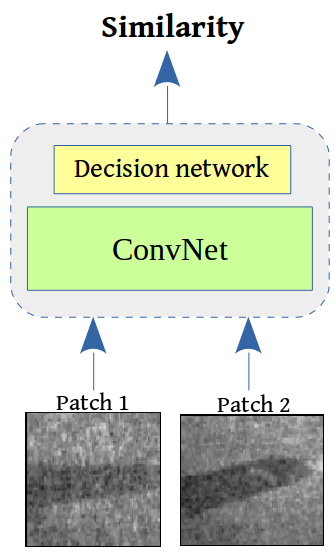
\includegraphics[width=4cm]{images/densenet/similarity_fn_grey}
\caption{Use of convolutional network for learning general similarity function for image patches. The patches in the image are samples taken from the data used in this thesis. 
Inspired from Zagoruyko et al.\cite{zagoruyko2015learning}}
\label{similarity_function_wraped}
\end{wrapfigure} 

For performing the patch matching task without using any hand designed features such as SIFT \cite{lowe2004distinctive}, we need to encode a network to learn the general
similarity function (figure \ref{similarity_function_wraped})
for sonar image patches. Which enables the network to predict that two input sonar patches contain different views of the same object or not i.e matching or non-matching respectively.

With the goal of obtaining the best possible result in the evaluation, best hyperparameters are needed to be found out.
The hyperparameters are the parameters of the network or learning process whose values are already set before the training starts \cite{wikihyper}. For example, the starting learning rate or the optimizer can be fixed before the training process starts. 

\subsection{Objectives}

\begin{enumerate}
 \item Select and evaluate a number of state of the art architectures which can perform sonar patch matching more effectively and improve the state of the art result (table \ref{best_results_stateoftheart}). The dataset presented in 
 \cite{stateoftheart} is used for evaluating different architectures. 
 \item Through grid search, determining the best hyperparameters for each of the architectures is a very important part of this work.
 \item Another objective is to present a comparative analysis of the performance of all the architectures. The metric of comparison is the ROC area under the curve value of the prediction score computed on the test dataset (D) from Valdenegro et al 
 \cite{stateoftheart}.
\end{enumerate}


The structure of the report is as follows. In the State of the art chapter \ref{chap:state} the related works that are done is presented. In Methodology chapter \ref{chap:method} the data and architectures evaluated are presented in details. The Evaluation chapter contains details of how the grid search was performed for finding best hyperparameters. Then in Results chapter the best hyperparameters search results and eventually best hyperparameters for each of the architecture and their best prediction
on the test data is presented. The Results section ends with comparative analysis of all the architectures evaluated. Lastly, in Conclusions, the contribution of this work, future research directions etc. are discussed.
